% ============================================================
%  MÓDULO 01 — Capa, Folha de Rosto e Sumário
% ============================================================
% ============================================================
%  MÓDULO 01 — Capa, Prefácio, Folha de Rosto e Sumário
% ============================================================
\thispagestyle{empty}
\pagestyle{empty}
% --- Capa (página 1) -----------------------------------------
% R621: a capa passa a ser a arte_final do autor (monografia "OpenCode
% Ecosystem v5.1.0", fonte: PDF Canva do próprio autor). Substitui a capa
% desenhada em TikZ que vigorou de R599 a R620. A arte é raster em A4 cheio
% (1755x2483 px, ~213 dpi): entra como imagem, não como texto, para que a
% diagramação do PDF de origem não seja reinterpretada nem recomposta.
\noindent
\begin{tikzpicture}[remember picture,overlay]
  \node[inner sep=0,anchor=center] at (current page.center)
    {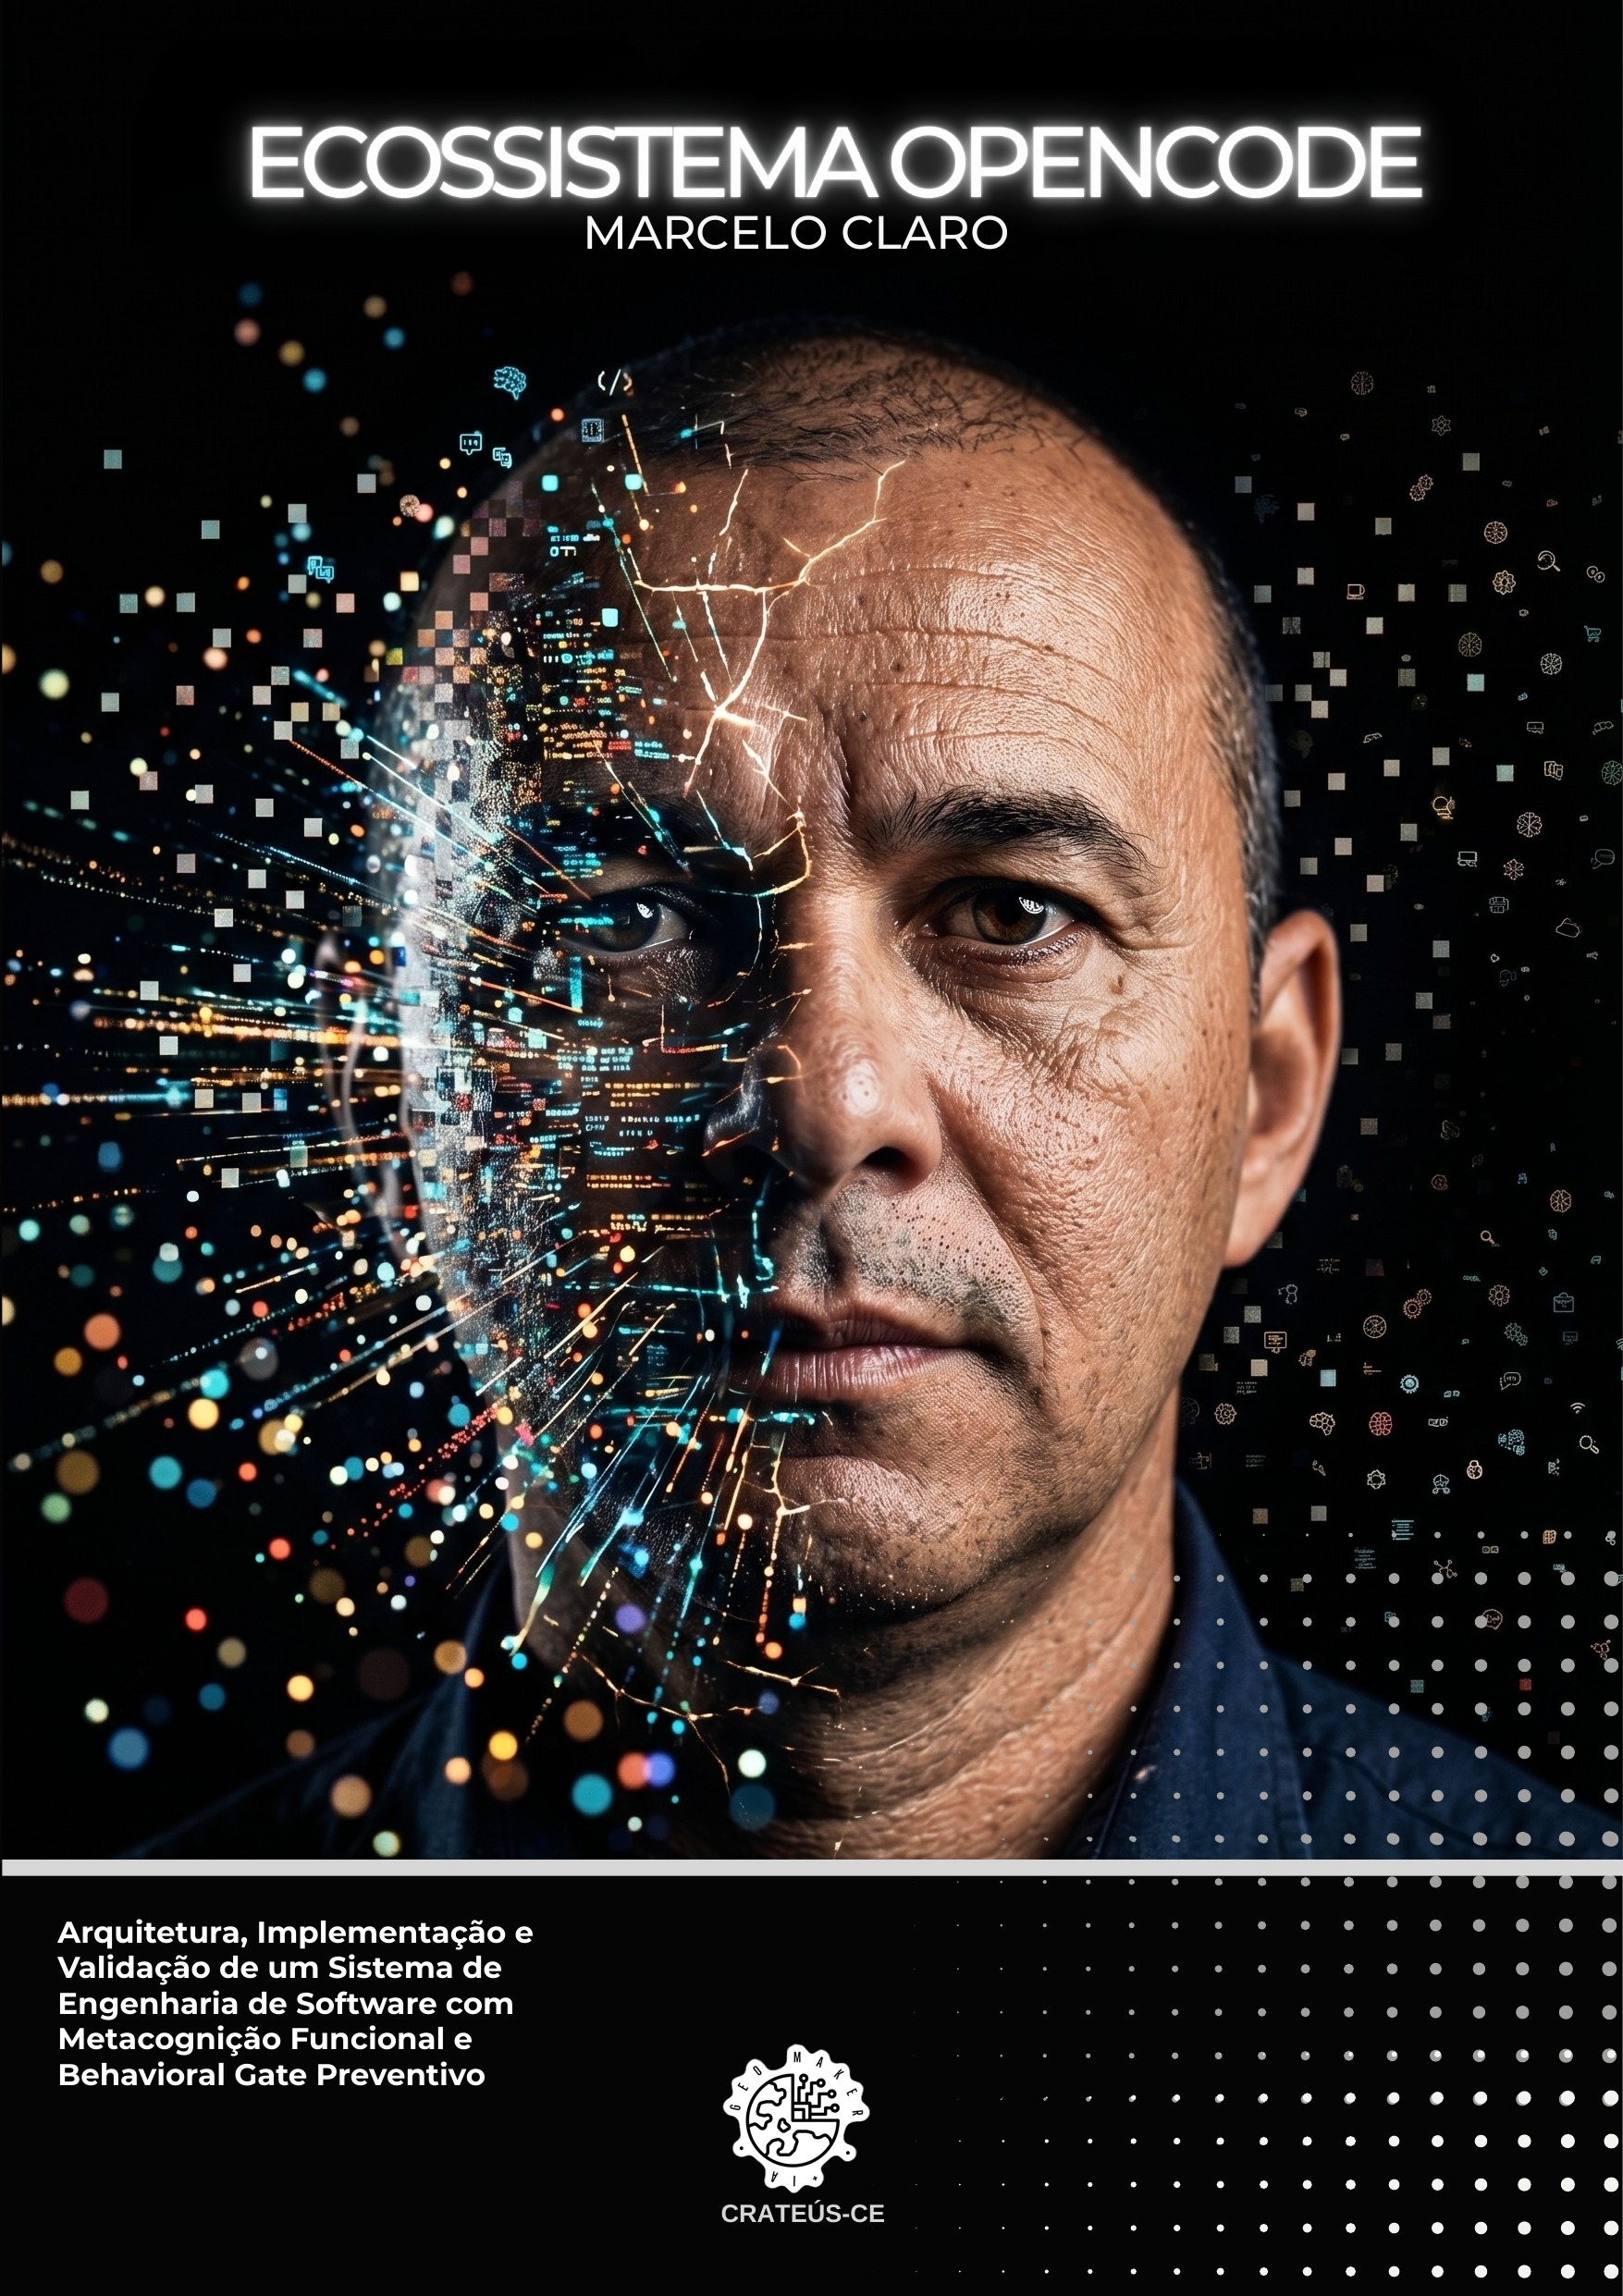
\includegraphics[width=\paperwidth,height=\paperheight]{capa-ecosistema.jpg}};
\end{tikzpicture}%
\null
\clearpage
\pagestyle{fancy}

% --- Prefácio (nota do autor) ---------------------------------
% R621: texto "NOTA DO AUTOR PARA ESTE LIVRO" do PDF do autor, verbatim.
% Mantido como prefácio e não como peça editorial do Core: a voz é a do autor.
\begin{flushleft}
 {\small\sffamily\color{plumAccent}\MakeUppercase{OpenCode Ecosystem Core}\par}
\vspace{2mm}
 {\Large\sffamily\bfseries\color{textmain}Prefácio --- Nota do autor para este livro\par}
{\color{plumAccent}\rule{0.25\linewidth}{1.2pt}\par}
\end{flushleft}
\vspace{2mm}
\begin{elemento}{Nota do autor}{\metainfo{ID}{PREF-01} \hfill \metainfo{Fonte}{arte final do autor} \hfill \metainfo{Ciclo}{R621}}
Este livro nasceu de uma necessidade: democratizar o conhecimento sobre arquitetura de sistemas multiagente. Não basta saber usar IA --- é preciso entender como ela pensa. O ECOSSISTEMA OpenCode é resultado de anos de pesquisa, experimentos e, principalmente, da convicção de que qualquer educador pode construir suas próprias ferramentas.

Dedico este trabalho a todos os professores que, como eu, acreditam que a tecnologia deve servir para ampliar --- nunca substituir --- o potencial humano de criar, questionar e transformar.

Obrigado por fazer parte desta jornada.
\begin{flushright}
--- Marcelo Claro Laranjeira.\\ Crateús, Ceará, 2026.
\end{flushright}
\end{elemento}
\clearpage

% --- Folha de rosto ------------------------------------------
\thispagestyle{plain}
\vspace*{0.20\paperheight}
\begin{center}
\sffamily
{\color{plumAccent}\rule{0.16\linewidth}{1.4pt}}\\[8pt]
{\small\bfseries\color{steel}\MakeUppercase{Série técnica e científica}}\\[12pt]
{\fontsize{25}{29}\selectfont\bfseries\color{textmain}Manual Técnico-Dev-Científico\\[3pt]do OpenCode Ecosystem Core}\\[10pt]
{\color{plumAccent}\rule{0.32\linewidth}{0.8pt}}\\[12pt]
{\large\color{textmuted}Elemento, agente e subagente: ficha de raio-x com descrição, conceito, cálculo,\\
fluxo de trabalho, interações, impacto, limites, arquitetura e fluxograma}\\[22pt]
\begin{tcolorbox}[width=0.9\linewidth,colback=panel,colframe=plumAccent,boxrule=0.6pt,arc=1.5mm,left=5mm,right=5mm,top=4mm,bottom=4mm]
{\small Coordenação do ecossistema: \textbf{MarceloClaro Orchestrator} (proto-coordenação A2A/MetaBus)\\[3pt]
Autor/organizador: \textbf{Marcelo Claro Laranjeira} \;$\cdot$\; ORCID \href{https://orcid.org/0000-0001-8996-2887}{0000-0001-8996-2887} \;$\cdot$\; \texttt{marceloclaro@gmail.com}\\[3pt]
Rigor: protocolos SDD/TDD + política anti-overclaim (CORRIGENDUM)\\[3pt]
Ferramenta de geração: LaTeX (pdf\TeX)}
\end{tcolorbox}
\vspace{14pt}
{\small\itshape\color{textmuted}Livro documental elaborado a partir da leitura do código-fonte, catálogos, especificações,\\
registros de evolução, testes e mapa do ecossistema (MAPA\_ECOSSISTEMA\_COMPLETO).}
\end{center}
\vfill
{\small\sffamily\centering Nenhuma afirmação deste manual deve ser lida como mérito de qualidade externa\\[1pt]
(Qualis A1, benchmark, "superhuman") sem validação externa explícita — ver CORRIGENDUM.\par}
\clearpage

% --- Sumário -------------------------------------------------
\tableofcontents
\clearpage
